%\begin{figure}[H]
%    \centering
    \begin{tikzpicture}
        \pgfplotsset{
            width=1.0\textwidth,
            height=0.4\textheight
        }
        \begin{axis}
            [
                xbar=2pt,
                legend style={at={(0.5,-0.15)}, anchor=north,legend columns=-1},
                bar width = 5pt,
                xlabel= Execution Time (s),
                ylabel= Core,
                xmin=0,xmax=60,
                    ytick={0,1,2,3,4,5,6,7,8,9},
            ]
            \addplot coordinates { 
                (11.89,0)
                (11.48,1)
                (11.48,2)
                (11.46,3)
                (11.46,4)
                (11.48,5)
                (29.61,6)
                (29.58,7)
                (29.58,8)
                (29.59,9)
                };
            \addplot coordinates { 
                (14.005,0)
                (13.98,1)
                (13.98,2)
                (13.98,3)
                (13.98,4)
                (13.96,5)
                (58.92,6)
                (58.92,7)
                (58.92,8)
                (58.93,9)
                };
            \legend{NB, SN}
            \end{axis}
        \end{tikzpicture}
    \caption{Execution time}
    % \caption{The Execution Time for DUT 2, where both benchmarks are compiled on oneAPI}
%\end{figure}
